\documentclass[../main.tex]{subfiles}
\graphicspath{{\subfix{../figures/}}}
%
\begin{document}
\section{享元模式(Flyweight)}
\textbf{享元模式的用意}:
享元模式是对象的结构模式. 享元模式以共享的方式高效地支持大量的细粒度对象的维护与管理.
享元对象能实现共享的关键是区分\textbf{内部状态}(Internal  state)和\textbf{外部状态}(External State).

\textbf{内部状态}是存储在享元对象内部的并且是不会随环境改变而有所不同的.因此,一个享元可以具有内部状态并可以共享.

\textbf{外部状态}是随环境改变而改变的、不可以共享的状态.享元对象的外部状态必须由客户端保存,并在享元对象被创建之后,在需要使用的时候再传入到享元对象内部.
外部状态不可以影响享元对象的内部状态.内外部状态是互相独立的.

\textbf{享元模式的种类}:
根据所涉及的享元对象的内部结构,享元模式可以分成\textbf{单纯享元模式}
和\textbf{复合享元模式}两种形式.下图是单纯享元模式的结构示意图:
%
\begin{figure}[H]
  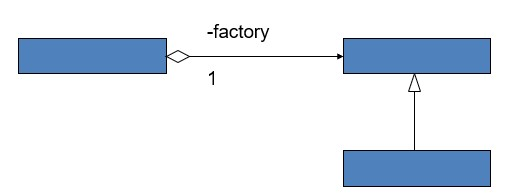
\includegraphics[width=0.45\textwidth]{24_1.jpg}
\end{figure}
%
下图所示是复合享元模式的结构示意图:
%
\begin{figure}[H]
  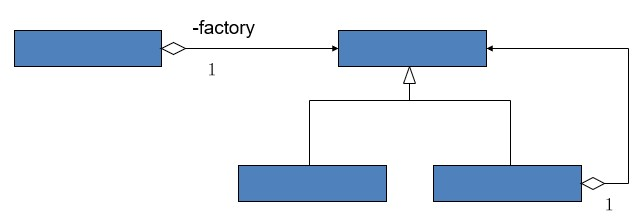
\includegraphics[width=0.45\textwidth]{24_2.jpg}
\end{figure}
%
可见,在复合享元模式中,享元对象构成合成模式.因此,\textbf{复合享元模式}实际上是\textbf{单纯享元模式}与\textbf{合成模式}的组合。

\textbf{享元模式的应用}:
\begin{itemize}
  \item 享元模式在编辑器系统中大量使用.一个文本编辑器往往会提供很多种字体,而通常的做法就是将每一个字母作成一个享元对象.享元对象的内部状态就是这个字母的字符数据,而字母在文本中的位置和字体风格等其它信息则是外部状态.
  \item 在Java语言中,String类型就使用了享元模式.String对象是不变对象,一旦创建出来就不能改变.
\end{itemize}
%
\subsection{单纯享元模式的结构}

\end{document}
